\section{Introduction}


The nearest neighbor search problem is defined as follows: given a set $X$ of $n$ points in a $d$-dimensional space, build a data structure that, given any query point $y$, returns the point in $X$ closest to $y$. For efficiency reasons, the problem is often relaxed to approximate nearest neighbor search, where the goal is to find a point $x \in X$ whose distance to $y$ is at most $c \min_{x \in X} \|x-y\|$ for some approximation factor $c>1$. Both problems have found numerous applications in machine learning, computer vision,  information retrieval and other areas. In machine learning in particular, nearest neighbor classifiers are popular baseline methods whose classification error often comes close to that of the best known techniques (\cite{efros}).

%https://nn2017.mit.edu/wp-content/uploads/sites/5/2017/12/Efros-NIPS-NN-17.pdf

Developing fast approximate nearest neighbor search algorithms have been a subject of extensive research efforts over the last last two decades, see  e.g.,~\cite{shakhnarovich2006nearest,AI} for an overview.  More recently, there has been increased focus on  designing nearest neighbor methods that use a limited amount of {\em space}. This is motivated by the need to fit  the data set in the main memory (\cite{johnson2017billion,faiss}) or an Internet of Things device (\cite{gupta2017protonn}).  Furthermore, even a simple linear scan over the data is more time-efficient if the data is compressed. 
The data set compression is most often achieved 
% by sparsifying the original data set [ProtoNN] or 
by developing compact representations of data that approximately preserve the distances between the points (see~\cite{wang2016learning} for a survey). 
%Exam such as ~\cite{broder1997resemblance, indyk1998approximate, kushilevitz2000efficient, torralba2008small, weiss2009spectral, jegou2011product, norouzi2012hamming, shrivastava2014densifying}
Such representations are smaller than the original (uncompressed) representation of the data set, while  approximately preserving the distances between points.  

Most of the approaches in the literature are only validated empirically.
%(eg.~the surveys~\cite{wang2016learning}, \cite{wang2018survey}).
The currently best known {\em theoretical} tradeoffs between the representation size and the approximation quality are summarized in Table~\ref{tbl:sketches_related_work}, together with their functionalities and constraints. 
\begin{table}[h]
\begin{center}
\begin{tabular}{| l | l | l |}
\hline
& 		Bits per point	& Comments \\
\hline
No compression 		& $d  \log n$ 							&  \\
\cite{johnson1984extensions}	& $\epsilon^{-2} \log^2(n)$			& Estimates distances between any $y$ and all $x \in X$\\
 \cite{kushilevitz2000efficient}				& $\epsilon^{-2} \log(n) \log (R)$				& Estimates distances between any $y$ and all $x \in X$,  \\
 & & assuming $\|x-y\| \in [r, R r]$ \\
 \cite{indyk2017near}				& $\epsilon^{-2} \log(n) \log(1/\epsilon)$	& Estimates distances between all $x,y \in X$,  \\
 & & does not provably support out-of-sample queries \\
 \hline
 This paper			& $\epsilon^{-2} \log(n) \log(1/\epsilon)$      & Returns an approximate nearest neighbor of $y$ in $X$\\
 \hline
\end{tabular}
\caption{Comparison of Euclidean metric sketches with distortion $1\pm\epsilon$. We assume that all point coordinates are represented using $\log \Phi$ bits, or alternatively that each coordinate is an integer in the range $\{ -\Phi \ldots \Phi\}$.
For the sake of exposition, the results depicted in the table assume $\Phi=n^{O(1)}$. Furthermore, the compression algorithm can be randomized, and the compressed representation must enable approximating distances up to a factor of $1 \pm \epsilon$ with probability $1/n^{O(1)}$. 
%for $d=O(\epsilon^{-2}\log n)$ and $\log\Phi=O(\log n)$.
}
\label{tbl:sketches_related_work}
\end{center}
\end{table}

Unfortunately,  in the context of approximate nearest neighbor search, the above representations lead to sub-optimal results. 
The result from the last row of the table (from \cite{indyk2017near}) cannot be used to obtain provable bounds for nearest neighbor search, because the distance preservation guarantees hold only for pairs of points in the pointset $X$.\footnote{We note, however, that a simplified version of this method, described in~\cite{indyk2017practical}, was shown to have  good empirical performance for nearest neighbor search.} 
The second-to-last result (from \cite{kushilevitz2000efficient}) only estimates distances in a certain range; extending this approach to all distances would multiply the storage by a factor of $\log \Phi$.  Finally,  the representations obtained via a direct application of  randomized dimensionality reduction (\cite{johnson1984extensions}) are also larger than the bound from~\cite{indyk2017near} by almost a factor of $\log \Phi$. 

\paragraph{Our results} In this paper we show that it is possible to overcome the limitations of the previous results and design a compact representation that supports $(1+\epsilon)$-approximate nearest neighbor search, with a space bound essentially matching that of~\cite{indyk2017near}. This constitutes the first reduction in the space complexity of approximate nearest neighbor below the  ``Johnson-Lindenstrauss bound''.
Specifically, we show the following. Suppose that we want the data structure to answer $q$ approximate nearest neighbor queries in a $d$-dimensional dataset of size $n$, in which coordinates are represented by $\log\Phi$ bits each.
All $q$ queries must be answered correctly with probability $1-\delta$. (See Section~\ref{s:formal} for the formal problem definition).

\begin{theorem}\label{thm:ann_ub}
For the all-nearest-neighbors problem, there is a sketch of size 
\[
  O\left( n\left(\frac{\log n\cdot\log(1/\epsilon)}{\epsilon^2} + \log\log\Phi + \log\left(\frac{q}{\delta}\right)\right) + d\log\Phi  + \log\left(\frac{q}{\delta}\right)\log\left(\frac{\log(q/\delta)}{\epsilon}\right) \right)
  \;\; \text{bits.}
\]
%\[ O(n(d+\log n)\log(1/\epsilon) + n\log\log\Phi + n\log(q/\delta) + \mathrm{poly}(d,\log\Phi,\log(q/\delta)) \;\; \text{bits.} \]
%where $q$ is the total number of queries, all of which .
\end{theorem}
The proof is given in~\Cref{sec:ann}. We also give a lower bound of
 $\Omega(n \log(n) /\epsilon^2)$ for $q=1$ and $\delta=1/n^{O(1)}$ (Section~\ref{sec:nnlower}), which shows that the first term in the above theorem is almost tight. 
 
Interestingly, the  representation by itself does not return the  (approximate) {\em distance} between the query point and the returned neighbor. 
%The aforementioned representation is able to report an approximate nearest neighbor for an out-of-sample query point, but not the distance between them.
Thus, we also consider the problem of estimating distances from a query point to all data points.
In this setting, a result of~\cite{molinaro2013beating} shows that the Johnson-Lindenstrauss space bound is optimal when the number of queries is~\emph{equal} to the number of data points.
However, in many settings, the number of queries is often substantially smaller than the dataset size.
We give nearly tight upper and lower bounds (up to a factor of $\log(1/\epsilon)$) for this problem, showing it is possible to smoothly interpolate between~\cite{indyk2017near}, which does not support out-of-sample distance queries, and the Johnson-Lindenstrauss bound. 
%See Section~\ref{s:formal} for the formal statements of all results. 

Specifically, we show the following. Suppose that we want the data structure to estimate all cross-distances between a set of $q$ queries and all points in $X$, all of which must be estimated correctly with probability $1-\delta$ (see Section~\ref{s:formal} for the formal problem definition).


\begin{theorem}\label{thm:distances_ub}
For the all-cross-distances problem, there is a sketch of size
\[ O\left(\frac{n}{\epsilon^2}\left(\log n\cdot\log(1/\epsilon) + \log(d\Phi)\log\left(\frac{q}{\delta}\right)\right) + \mathrm{poly}(d,\log\Phi,\log(q/\delta),\log(1/\epsilon))\right) \;\;  \text{bits.} \]
%where $q$ is the total number of queries, all of which must succeed with probability $1-\delta$.
\end{theorem}
Note that  the dependence per point on $\Phi$ is logarithmic, as opposed to doubly logarithmic in Theorem~\ref{thm:ann_ub}.
% The proof is given in~\Cref{sec:dist}.
We show this dependence is necessary, as per the following theorem. 
%complement the upper bound by showing the following. 
\begin{theorem}\label{thm:distances_lb}
Suppose that $d^{1-\rho}\geq\epsilon^{-2}\log(nq/\delta)$, $\Phi\geq1/\epsilon$, and $1/n^{0.5-\rho'}\leq\epsilon\leq\epsilon_0$ for some constants $\rho,\rho'>0$ and a sufficiently small constant $\epsilon_0$.
Then, for the all-cross-distances problem, any sketch must use at least
\[ \Omega\left(\frac{n}{\epsilon^2}\left(\log n + \log(d\Phi)\log\left(\frac{q}{\delta}\right)\right)\right) \;\; \text{bits.} \]
\end{theorem}
The proofs are given in ~\Cref{sec:dist} and \Cref{sec:dist_lb}, respectively. 

\paragraph{Practical variant}
\cite{indyk2017practical} presented a simplified version of~\cite{indyk2017near}, which has slightly weaker size guarantees, but on the other hand is practical to implement and was shown to work well empirically.
However, it did not provably support out-of-sample queries.
Our techniques in this paper can be adapted to their algorithm and endow it with such provable guarantees, while retaining its simplicity and practicality. We elaborate on this in Appendix~\ref{sec:middleout}.

\paragraph{Our techniques}
The starting point of our representation is the compressed tree data structure from~\cite{indyk2017near}.  The structure is obtained by constructing a hierarchical clustering of the data set, forming a tree of clusters.  The position of each point corresponding to a node in the tree is then represented by storing a (quantized) displacement vector between the point and its ``ancestor'' in the tree.
The resulting tree is further compressed by identifying and post-processing ``long'' paths in the tree. 
The intuition is that a subtree at the bottom of such a path corresponds to a cluster of points that is ``sufficiently separated'' from the rest of the points (see Figure~\ref{fig:noquery}). This means that the data structure does not need to know the exact position of this cluster in order to estimate the distances between the points in the cluster and the rest of the data set. Thus the data structure replaces each long path by a quantized displacement vector, where the quantization error does not depend on the length of the path. This ensures that the tree does not have long paths, which bounds its total size. 
% together with and approximates the rest of the path by an appropriately quantized displacement vector. 

Unfortunately, this reasoning breaks down if one of the points  is not known in advance, as it is the case for the approximate nearest neighbor problem. In particular, if the query point $y$ lies in the vicinity of the separated cluster, then small perturbations to the cluster position can dramatically affect which points in the cluster are closest to $y$ (see Figure~\ref{fig:query} for an illustration). 

In this paper we overcome this issue by maintaining extra information about the geometry of the point set. First, for each long path, we store not only the quantized displacement vector (which preserves the ``global'' position of the subtree with respect to the rest of the tree) but also the {\em suffix} of the path. Intuitively, this allows us to recover both the {\em most} significant bits and the {\em least} significant bits of  points in the subtree corresponding to the ``separated" clusters, which allows us to avoid cases as depicted in Figure~\ref{fig:query}. However, this intuition breaks down when the diameter of the cluster is much larger than the amount of ``separation".  Thus we also need to store extra information about the position of the subtree points. This is accomplished by storing a hashed representation of a representative point of the subtree (called ``the center"). We note that this modification makes our data structure inherently randomized; in contrast, the data structure of~\cite{indyk2017near} was deterministic.
% even though it was constructed using the probabilistic method.

Given the above information, the approximate nearest neighbor search is performed top down, as follows. In each step, we recover and enumerate points  in the current subtree, some of which could be centers of ``separated'' clusters as described above. The ``correct'' center, guaranteed to contain an approximate nearest neighbor of the query point, is identified by its hashed value (if no hash match is found, then any center is equally good). Note that our data structure does not allow us to compute all distances from the query point $y$ to all points in $X$ (in fact, as mentioned earlier, this task is not possible to achieve within the desired space bound). Instead, it stores just enough information to ensure that the procedure never selects a ``wrong" subtree to iterate on.

Lastly, suppose we also wish to estimate all distances from $y$ to $X$.
To this end, we augment each subtree with the distance sketches due to~\cite{kushilevitz2000efficient} and~\cite{johnson1984extensions}.
The former allows us to identify the cluster of~\emph{all} approximate nearest neighbors of $y$ (whereas the above algorithm was only guaranteed to return~\emph{one} approximate nearest neighbor).
The latter stores the approximate distance from that cluster.
These are the smallest distances from $y$ to $X$, which are the most challenging to estimate; the remaining distances can be estimated based on the hierarchical partition into well-separated clusters, which is already present in the sketch.

\begin{figure}[t]
\vskip 0.2in
\begin{center}
%\centerline{\includegraphics[scale=0.6]{decompression_noquery}}
\centerline{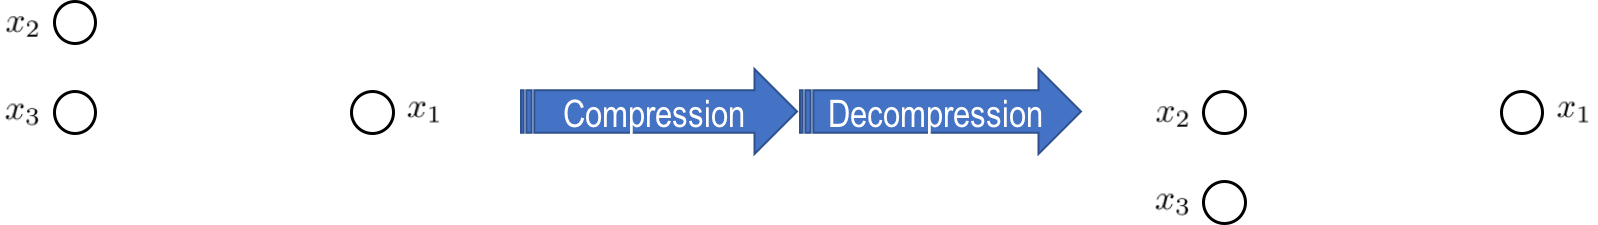
\includegraphics[scale=0.5]{clusters_noquery_cd}}
\caption{Compression and decompression of a two-dimensional dataset. The location of the well-separated cluster $\{x_2,x_3\}$ can be perturbed by the lossy compression algorithm, without significantly changing the distances to $x_1$.}
\label{fig:noquery}
\end{center}
\vskip -0.2in
\end{figure} 

\begin{figure}
\vskip 0.2in
\begin{center}
%\centerline{\includegraphics[scale=0.6]{decompression_query}}
\centerline{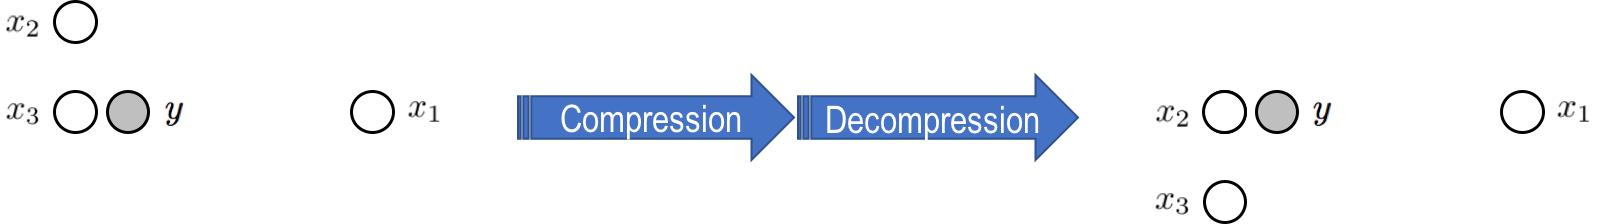
\includegraphics[scale=0.5]{clusters_query_cd}}
\caption{Compression and decompression of a dataset $x_1,x_2,x_3$ in the presence of a new query point $y$, which is unknown during compression. The same small perturbation in the location of $\{x_2,x_3\}$ as in Figure~\ref{fig:noquery} fails to preserve $x_3$ as the nearest neighbor of $y$.}
\label{fig:query}
\end{center}
\vskip -0.2in
\end{figure} 
